\documentclass[10pt]{beamer}

\usetheme{metropolis}

\usepackage[utf8]{inputenc}
\usepackage{multirow}
\usepackage{colortbl}
\usepackage{float}
\usepackage{graphicx}
\usepackage{hyperref}
\usepackage{amsmath}
\usepackage{subcaption}

\newcommand{\themename}{\textbf{\textsc{metropolis}}\xspace}


\title{Hierarchical Attention Networks for Document Classification}
\date{\today}
\author{Emilio Cecchini \\ \textit{emilio.cecchini@stud.unifi.it}}
\institute{Università degli Studi di Firenze}
\titlegraphic{\hfill
\includegraphics[height=1.5cm]{img/unifi_logo.eps}}

\setbeamertemplate{frame footer}{Hierarchical Attention Networks for Document Classification - Emilio Cecchini}
\metroset{progressbar=foot}


\begin{document}


\maketitle


\begin{frame}{Introduction}

\begin{itemize}
\item
The goal of this project is to replicate the experiments of the 2016 paper \cite{yang2016hierarchical}.
\item
The main topic of the paper is document classification.
\item
The thesis of the authors is that a better representation can be obtained by incorporating knowledge of document structure in the model architecture.
\item
They introduced a new architecture: the Hierarchical Attention Network (HAN)
\item
All the code used for the experiments are available at \url{https://github.com/ceccoemi/han}
\end{itemize}

\end{frame}


\begin{frame}{Recurrent Neural Networks}
\small{
\begin{itemize}
\item
A RNN is an extension of a conventional feedforward neural network, which is able to handle a variable-length sequence input.
\item
The RNN handles the variable-length input sequence by having a recurrent hidden state whose activation at each time is dependent on that of the previous time.
\end{itemize}

Given an input sequence $\mathbf{x}=\left(x_1, \dots, x_T\right)$, traditionally the RNN updates its recurrent hidden state $\mathbf{h}_t$ with

\begin{align}
\mathbf{h_t} = g\left(W\mathbf{x}_t + U\mathbf{h}_{t-1}\right)
\end{align}

where $g$ is a smooth, bounded function. Optionally, the RNN may have an output $\mathbf{y}$ which may again be of variable length.
}
\end{frame}


\begin{frame}{Recurrent Neural Networks}

\begin{itemize}
\item
Unfortunately, it has been observed that is difficult to train RNNs to capture long-term dependencies because the gradient tend to either vanish or explode.
\item
There have been two dominant approaches by which many researchers have tried to reduce the negative impacts of this issue:
\begin{itemize}
\item
Better learning algorithm (\textit{gradient clipping}, \textit{second-order methods})
\item
More sophisticated activation function consisting of affine transformation followed by a simple element-wise nonlinearity by using gating units (LSTM, GRU)
\end{itemize}
\end{itemize}

\end{frame}


\begin{frame}{LSTM unit and GRU}

\begin{itemize}
\item
The Long Short-Term Memory (LSTM) unit was introduced in 1997 by Hochreiter and Schmidhuber \cite{hochreiter1997long}.
\item
A Gated Recurrent Unit (GRU) was proposed in 2014 by Cho et al. \cite{cho2014properties}. It's a simplified version of the LSTM unit that doesn't have two separated memory cells.
\end{itemize}

%\begin{figure}
%\centering
%\begin{subfigure}{0.5\textwidth}
%\centering
%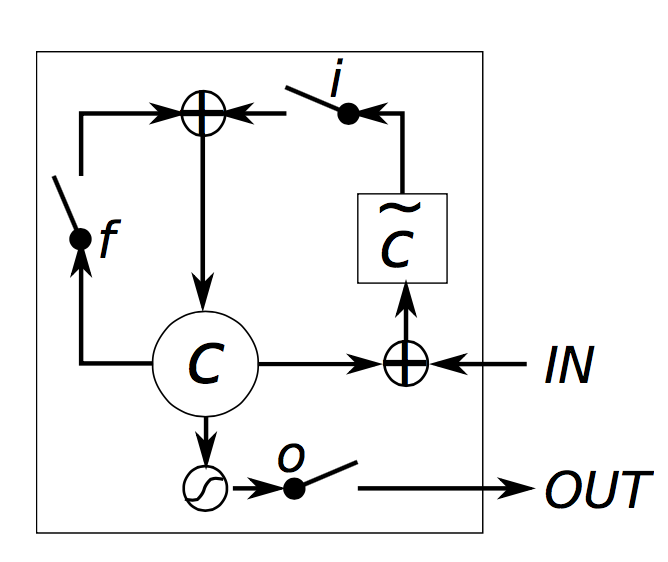
\includegraphics[scale=0.3]{img/lstm.png}
%\caption{\footnotesize{LSTM}}
%\end{subfigure}%
%~
%\begin{subfigure}{0.5\textwidth}
%\centering
%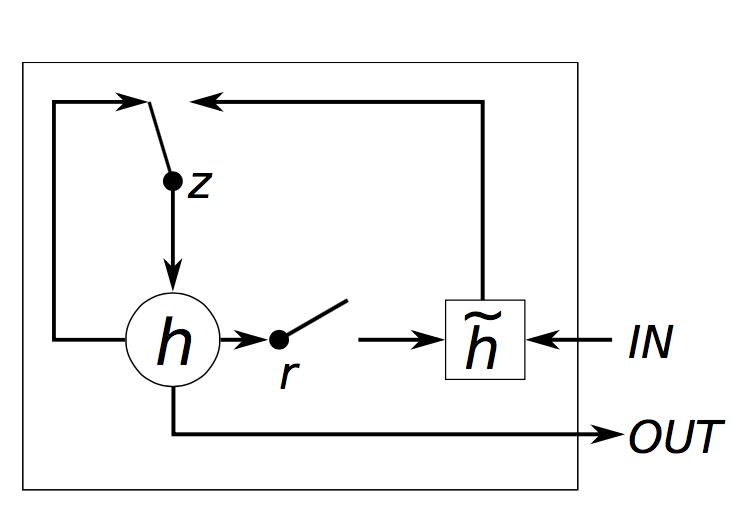
\includegraphics[scale=0.3]{img/gru.png}
%\caption{\footnotesize{GRU}}
%\end{subfigure}
%\end{figure}

\end{frame}


\begin{frame}{LSTM unit and GRU}

\begin{itemize}
\item
Chung et al. \cite{chung2014empirical} in 2014 demonstrated with various experiments that these two variations outperform the vanilla RNN units, but they weren't able to establish which of the two gating units was better.
\item
Greff et al. \cite{greff2016lstm} in 2017 evaluated eight different LSTM variations (including the GRU) and they concluded that the vanilla LSTM performs reasonably well on various data sets. However, the GRU simplifies the vanilla LSTM without significantly decreasing performance. The GRU can be preferred because it reduces the number of parameters and the computational cost.
\end{itemize}

\end{frame}


\begin{frame}{Attention mechanism}
\begin{itemize}
\item
Attention mechanism was first introduced by Bahdanau et al. in 2014 \cite{bahdanau2014neural} as a new encoder-decoder architecture in the topic of machine translation.
\item
The previously proposed encoder-decoder models encode a source sentence into a fixed-length vector from which a decoder generates a translation.
\item
Bahdanau et al. conjectured that the use of a fixed-length vector is a bottleneck in improving the performance of these models, so they proposed a new method that automatically (soft-)search for parts of a source sentence that are relevant to predict a target word.
\end{itemize}
\end{frame}


\begin{frame}{Attention mechanism}

\begin{itemize}
\item
The probability $\alpha_{i,j}$ reflects the importance of the annotation $h_j$ with respect to the previous hidden state $s_{i-1}$ in deciding the next state $s_i$, and generating $y_i$.
\item
The decoder decides parts of the source sentence to pay attention to.
\end{itemize}

\begin{figure}[H]
\centering
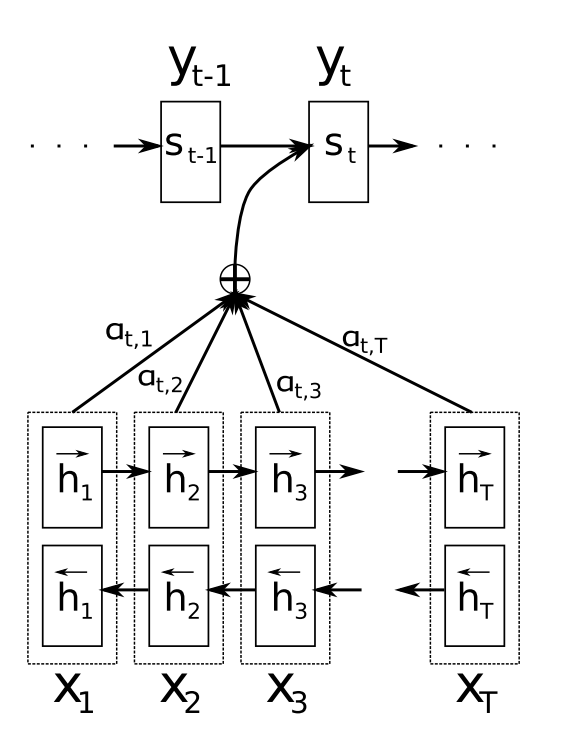
\includegraphics[scale=0.2]{img/attn.png}
\end{figure}

\end{frame}

\begin{frame}{Hierarchical Attention architecture}

\begin{figure}[H]
\centering
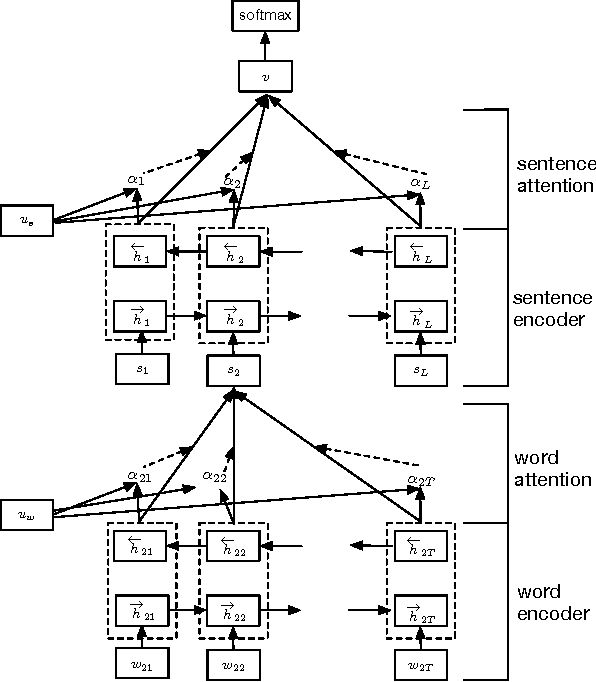
\includegraphics[scale=0.3]{img/hier_attn.png}
\label{graph_plot}
\end{figure}

\end{frame}


\begin{frame}{Word encoder}

\begin{itemize}
\item
Given the $i$th sentence of length $T$ with words $w_{it}, t \in [0,T]$, we first embed the words to vectors through a pretrained embedding matrix $W_e$.
\item
A bidirectional GRU is used to get words annotations $\overrightarrow{h_{it}}$ and $\overleftarrow{h_{it}}$, which are finally concatenated into a unique word annotation $h_{it}$, which summarizes the information of the whole sentence centered around $w_{it}$.\\
\end{itemize}
\begin{align*}
x_{it} &= W_ew_{it} \\
\overrightarrow{h_{it}} &= \overrightarrow{\operatorname{GRU}}(x_{it}) \\
\overleftarrow{h_{it}} &= \overleftarrow{\operatorname{GRU}}(x_{it}) \\
h_{it} &= [\overrightarrow{h_{it}}, \overleftarrow{h_{it}}]
\end{align*}

\end{frame}


\begin{frame}{Word attention}

\begin{itemize}
\item
The word annotation $h_{it}$ is fed through a one-layer MLP to get $u_{it}$.
\item
Then the importance of the word is measured with a word level context vector $u_w$. More precisely, a normalized importance $\alpha_{it}$ is obtained through a softmax function.
\item
Finally, a sentence vector $s_i$ is computed as a weighted sum of the word annotations and their importance.\\
\end{itemize}
\begin{align*}
u_{it} &= \tanh\left(W_wh_{it}+b_w\right) \\
\alpha_{it} &= \dfrac{\exp\left(u_{it}^Tu_{w}\right)}{\sum_t\exp\left(u_{it}^Tu_w\right)} \\
s_i &= \sum_t\alpha_{it}h_{it}
\end{align*}

\end{frame}


\begin{frame}{Sentence encoder}

\begin{itemize}
\item
Given the sentence vector $s_i$, a sentence annotation $h_i$ is obtained in the same way as the word encoder.
\item
A bidirectional GRU is used and a sentence annotation $h_i$ is obtained, which summarizes the neighbor sentences around sentence $i$ but still focus on sentence $i$.\\
\end{itemize}
\begin{align*}
\overrightarrow{h_{i}} &= \overrightarrow{\operatorname{GRU}}(s_{i}) \\
\overleftarrow{h_{i}} &= \overleftarrow{\operatorname{GRU}}(s_{i}) \\
h_{i} &= [\overrightarrow{h_{i}}, \overleftarrow{h_{i}}]
\end{align*}

\end{frame}


\begin{frame}{Sentence attention}

\begin{itemize}
\item
The same attention mechanism used for the words is introduced to get a word vector $v$ that summarizes all the information of the sentences in a document.\\
\end{itemize}
\begin{align*}
u_{i} &= \tanh\left(W_sh_i+b_s\right) \\
\alpha_{i} &= \dfrac{\exp\left(u_{i}^Tu_s\right)}{\sum_i\exp\left(u_i^Tu_s\right)} \\
v &= \sum_t\alpha_{i}h_{i}
\end{align*}

\end{frame}


\begin{frame}{Document classification}

\begin{itemize}
\item
Since the goal is document classification, a last step is required
\item
Given the document vector $v$, a probability vector $p$ is obtained with a MLP with a softmax activation:
\begin{align*}
p = \operatorname{softmax}\left(W_cv+b_c\right)
\end{align*}

\item
As training loss, a negative log likelihood is used:
\begin{align*}
L = -\sum_d\log p_{dj}
\end{align*}
\end{itemize}

\end{frame}


\begin{frame}{Data sets}

\begin{itemize}
\item
To evaluate the new proposed model, the authors used six different data sets: Yelp 2013, Yelp 2014, Yelp 2015, IMDB review, Yahoo answer and Amazon review.
\item
I choose three of the six dataset: Yelp, Yahoo and Amazon. Unfortunately, I wasn't able to find the exactly Yelp dataset used in the paper (while regarding Yahoo and Amazon I used the same data sets).
\item
Each data set is perfectly balanced and 80\% of the data is used for training, 10\% for validation and 10\% for test.
\end{itemize}

\begin{table}[]
\begin{tabular}{|c|c|c|}
\hline
\textbf{Data set} & \textbf{classes}  & \textbf{documents}  \\
\hline
Yelp & 5 & 700,000 \\
\hline
Yahoo answer & 10 & 1,450,000 \\
\hline
Amazon review & 5 & 3,650,000  \\
\hline
\end{tabular}
\end{table}

\end{frame}


\begin{frame}{Models}

\begin{itemize}
\item
The proposed model is compared with three other models:
\begin{itemize}
\item BoW (Bag-of-Words)
\item Flat Attention Network (FAN)
\end{itemize}
\end{itemize}

Note that the results of the FAN model is not reported in the paper.

\end{frame}


\begin{frame}{BoW}
\small{
\begin{itemize}
\item
The 50,000 most frequent words from the training set are selected and the count of each word is used as features.
\item
A Stochastic Gradient Descent classifier is used together with a logistic regression loss.
\item
A grid search cross-validation is used to find the best value for the regularization term $\alpha$.
\end{itemize}

\begin{table}[]
\begin{tabular}{c|c|c|}
\cline{2-3}
                       & \multicolumn{2}{c|}{\textbf{BoW}} \\
\hline
\multicolumn{1}{|c|}{\textbf{Data set}} & \textbf{Yang et al. \cite{yang2016hierarchical}} &  \textbf{Observed} \\
\hline
\multicolumn{1}{|c|}{Yelp} & 58.0 & 61.3 \\
\hline
\multicolumn{1}{|c|}{Yahoo} & 68.9 & 66.9 \\
\hline
\multicolumn{1}{|c|}{Amazon} & 54.4 & 52.2 \\
\hline
\end{tabular}
\caption{\small{Document classification, in percentage}}
\end{table}
}
\end{frame}


\begin{frame}{FAN and HAN}
\small{
\begin{itemize}
\item
Regarding model configuration, hyperparameters and training I tried to follow the setup reported in the paper. The only difference is that Yang et al. \cite{yang2016hierarchical} used grid search to find the best learning rate. Due to the high computational cost of the training I wasn't able to do that. I used a decresing learning rate instead.
\item
The embedding matrix was trained on the training and validation set. The word embedding dimension was set to 200.
\item
The GRU dimension was set to 50, so a bidirectional GRU gives 100 dimensions for word/sentence annotation.
\item
For training, a mini-batch size of 64 was used.
\item
The number of epochs are not specified in the paper. I choose to use early stopping with patience equals to 3.
\item
Stochastic gradient descent with momentum of 0.9 was used.
\end{itemize}
}
\end{frame}


\setbeamertemplate{frame footer}{}

\begin{frame}{Training (FAN model - Yelp)}

\begin{figure}[H]
\centering
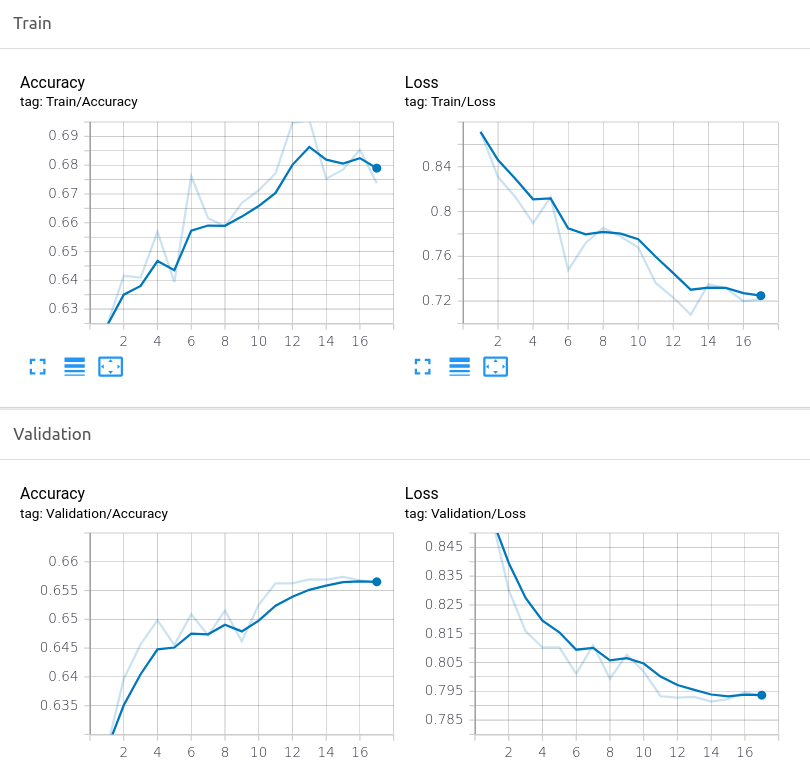
\includegraphics[scale=0.3]{img/yelp-fan.png}
\end{figure}

\end{frame}

\begin{frame}{Training (HAN model - Yelp)}

\begin{figure}[H]
\centering
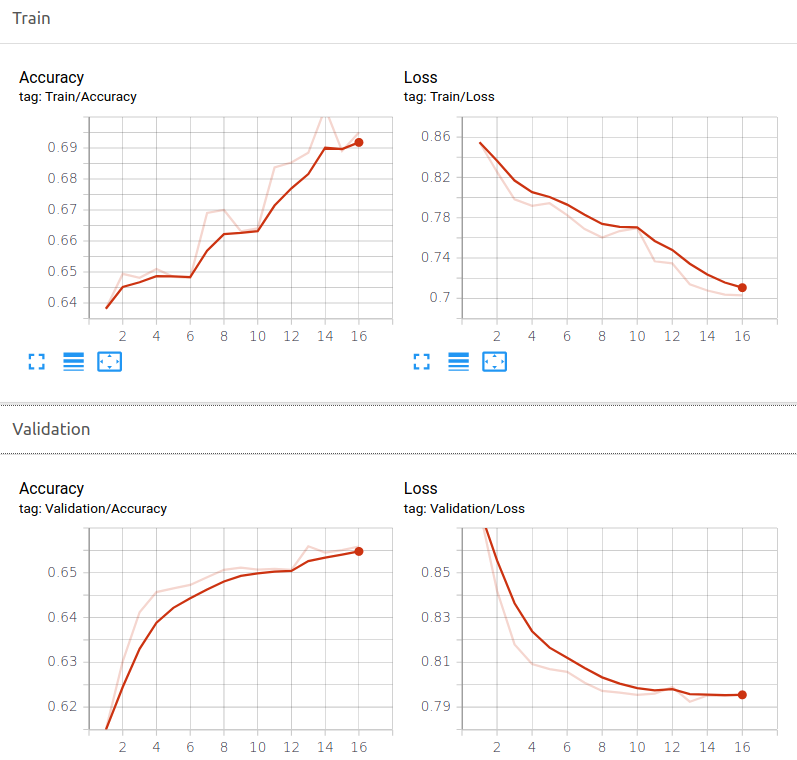
\includegraphics[scale=0.3]{img/yelp-han.png}
\end{figure}

\end{frame}

\begin{frame}{Training (FAN model - Yahoo)}

\begin{figure}[H]
\centering
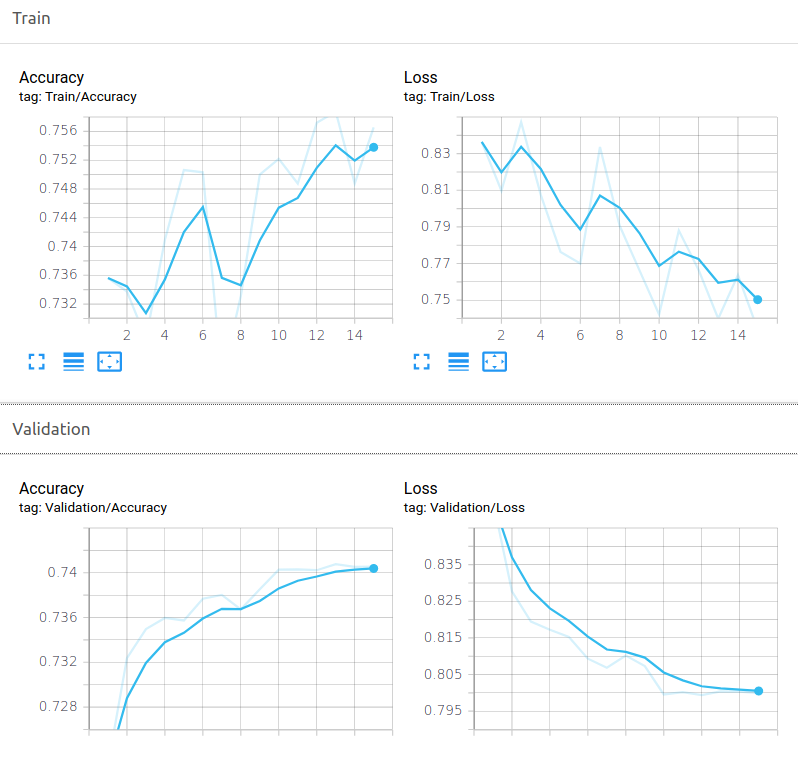
\includegraphics[scale=0.3]{img/yahoo-fan.png}
\end{figure}

\end{frame}

\begin{frame}{Training (HAN model - Yahoo)}

\begin{figure}[H]
\centering
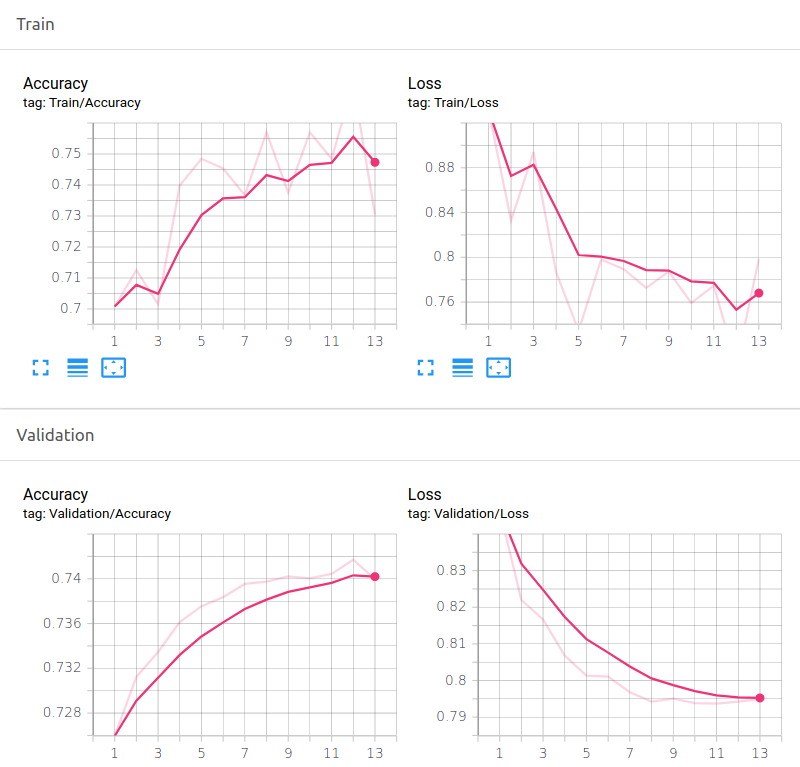
\includegraphics[scale=0.3]{img/yahoo-han.png}
\end{figure}

\end{frame}

\begin{frame}{Training (FAN model - Amazon)}

\begin{figure}[H]
\centering
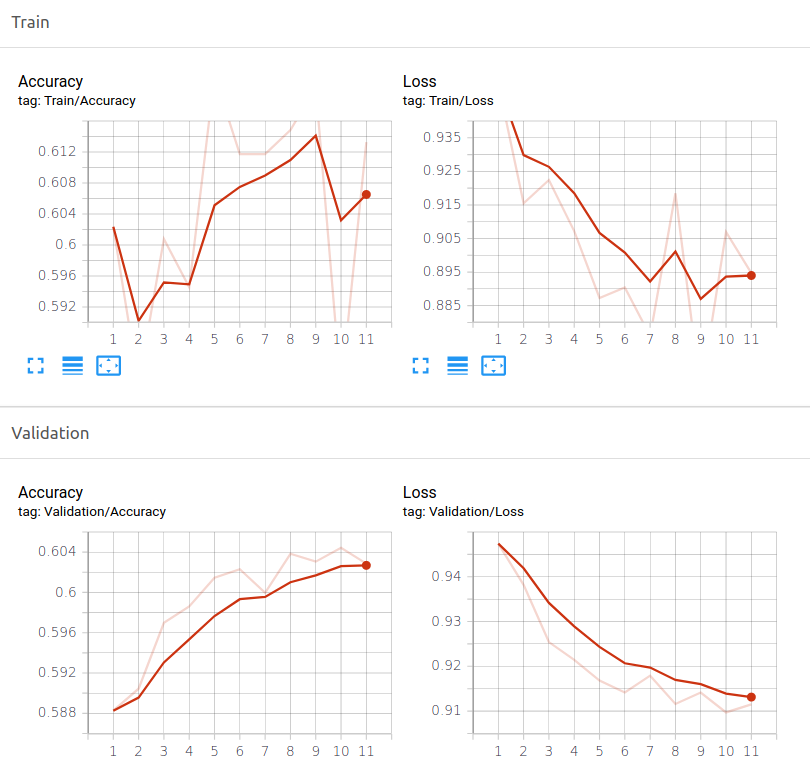
\includegraphics[scale=0.3]{img/amazon-fan.png}
\end{figure}

\end{frame}

\begin{frame}{Training (HAN model - Amazon)}

\begin{figure}[H]
\centering
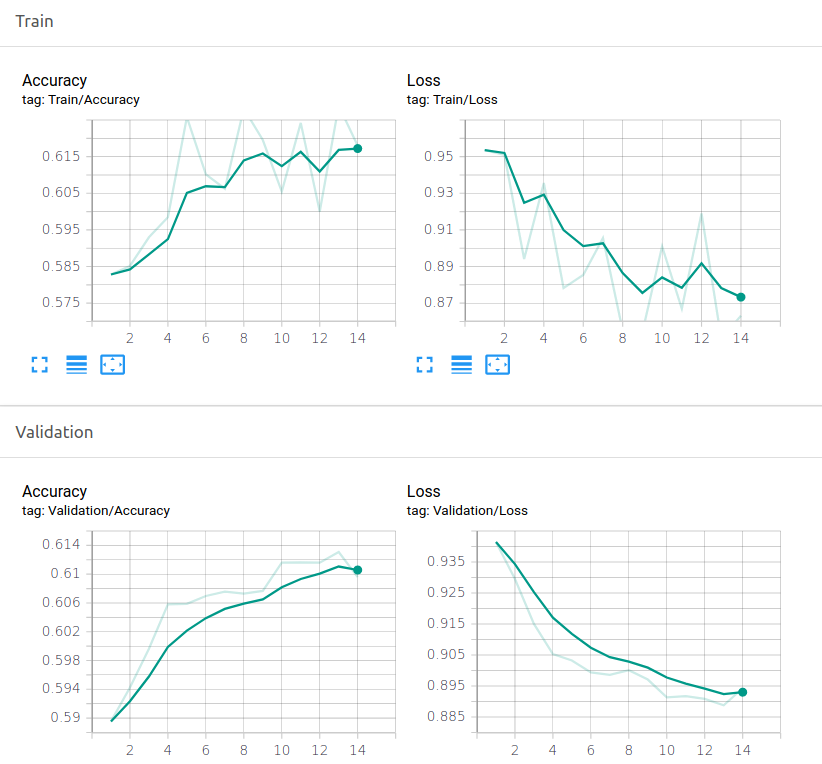
\includegraphics[scale=0.3]{img/amazon-han.png}
\end{figure}

\end{frame}

\setbeamertemplate{frame footer}{Hierarchical Attention Networks for Document Classification - Emilio Cecchini}

\begin{frame}{Experimental results}

\begin{table}[]
\begin{tabular}{c|c|c|c|}
\cline{2-4}
                       & \textbf{Flat attention (FAN)} & \multicolumn{2}{c|}{\textbf{Hierarchical attention (HAN)}} \\
\hline
\multicolumn{1}{|c|}{\textbf{Data set}} & \textbf{Observed} &  \textbf{Yang et al. \cite{yang2016hierarchical}} & \textbf{Observed} \\
\hline
\multicolumn{1}{|c|}{Yelp} & 65.6 & 68.2 & 65.6 \\
\hline
\multicolumn{1}{|c|}{Yahoo} & 74.1 & 75.8 & 74.4 \\
\hline
\multicolumn{1}{|c|}{Amazon} & 61.7 & 63.6 & 62.5 \\
\hline
\end{tabular}
\caption{\small{Document classification, in percentage}}
\end{table}

\end{frame}


\setbeamertemplate{frame footer}{}


\begin{frame}{Attention visualization}

\begin{itemize}
\item
An interesting feature of the attention mechanism is that it's easy to debug. That's because, as reported in the paper, you can easly visualize the how much importance each word and sentence has for the classification task.
\item
I've tried to reproduce this attention visualization.
\end{itemize}

\end{frame}


\begin{frame}{Yelp - Attention visualization}

\begin{figure}
\centering
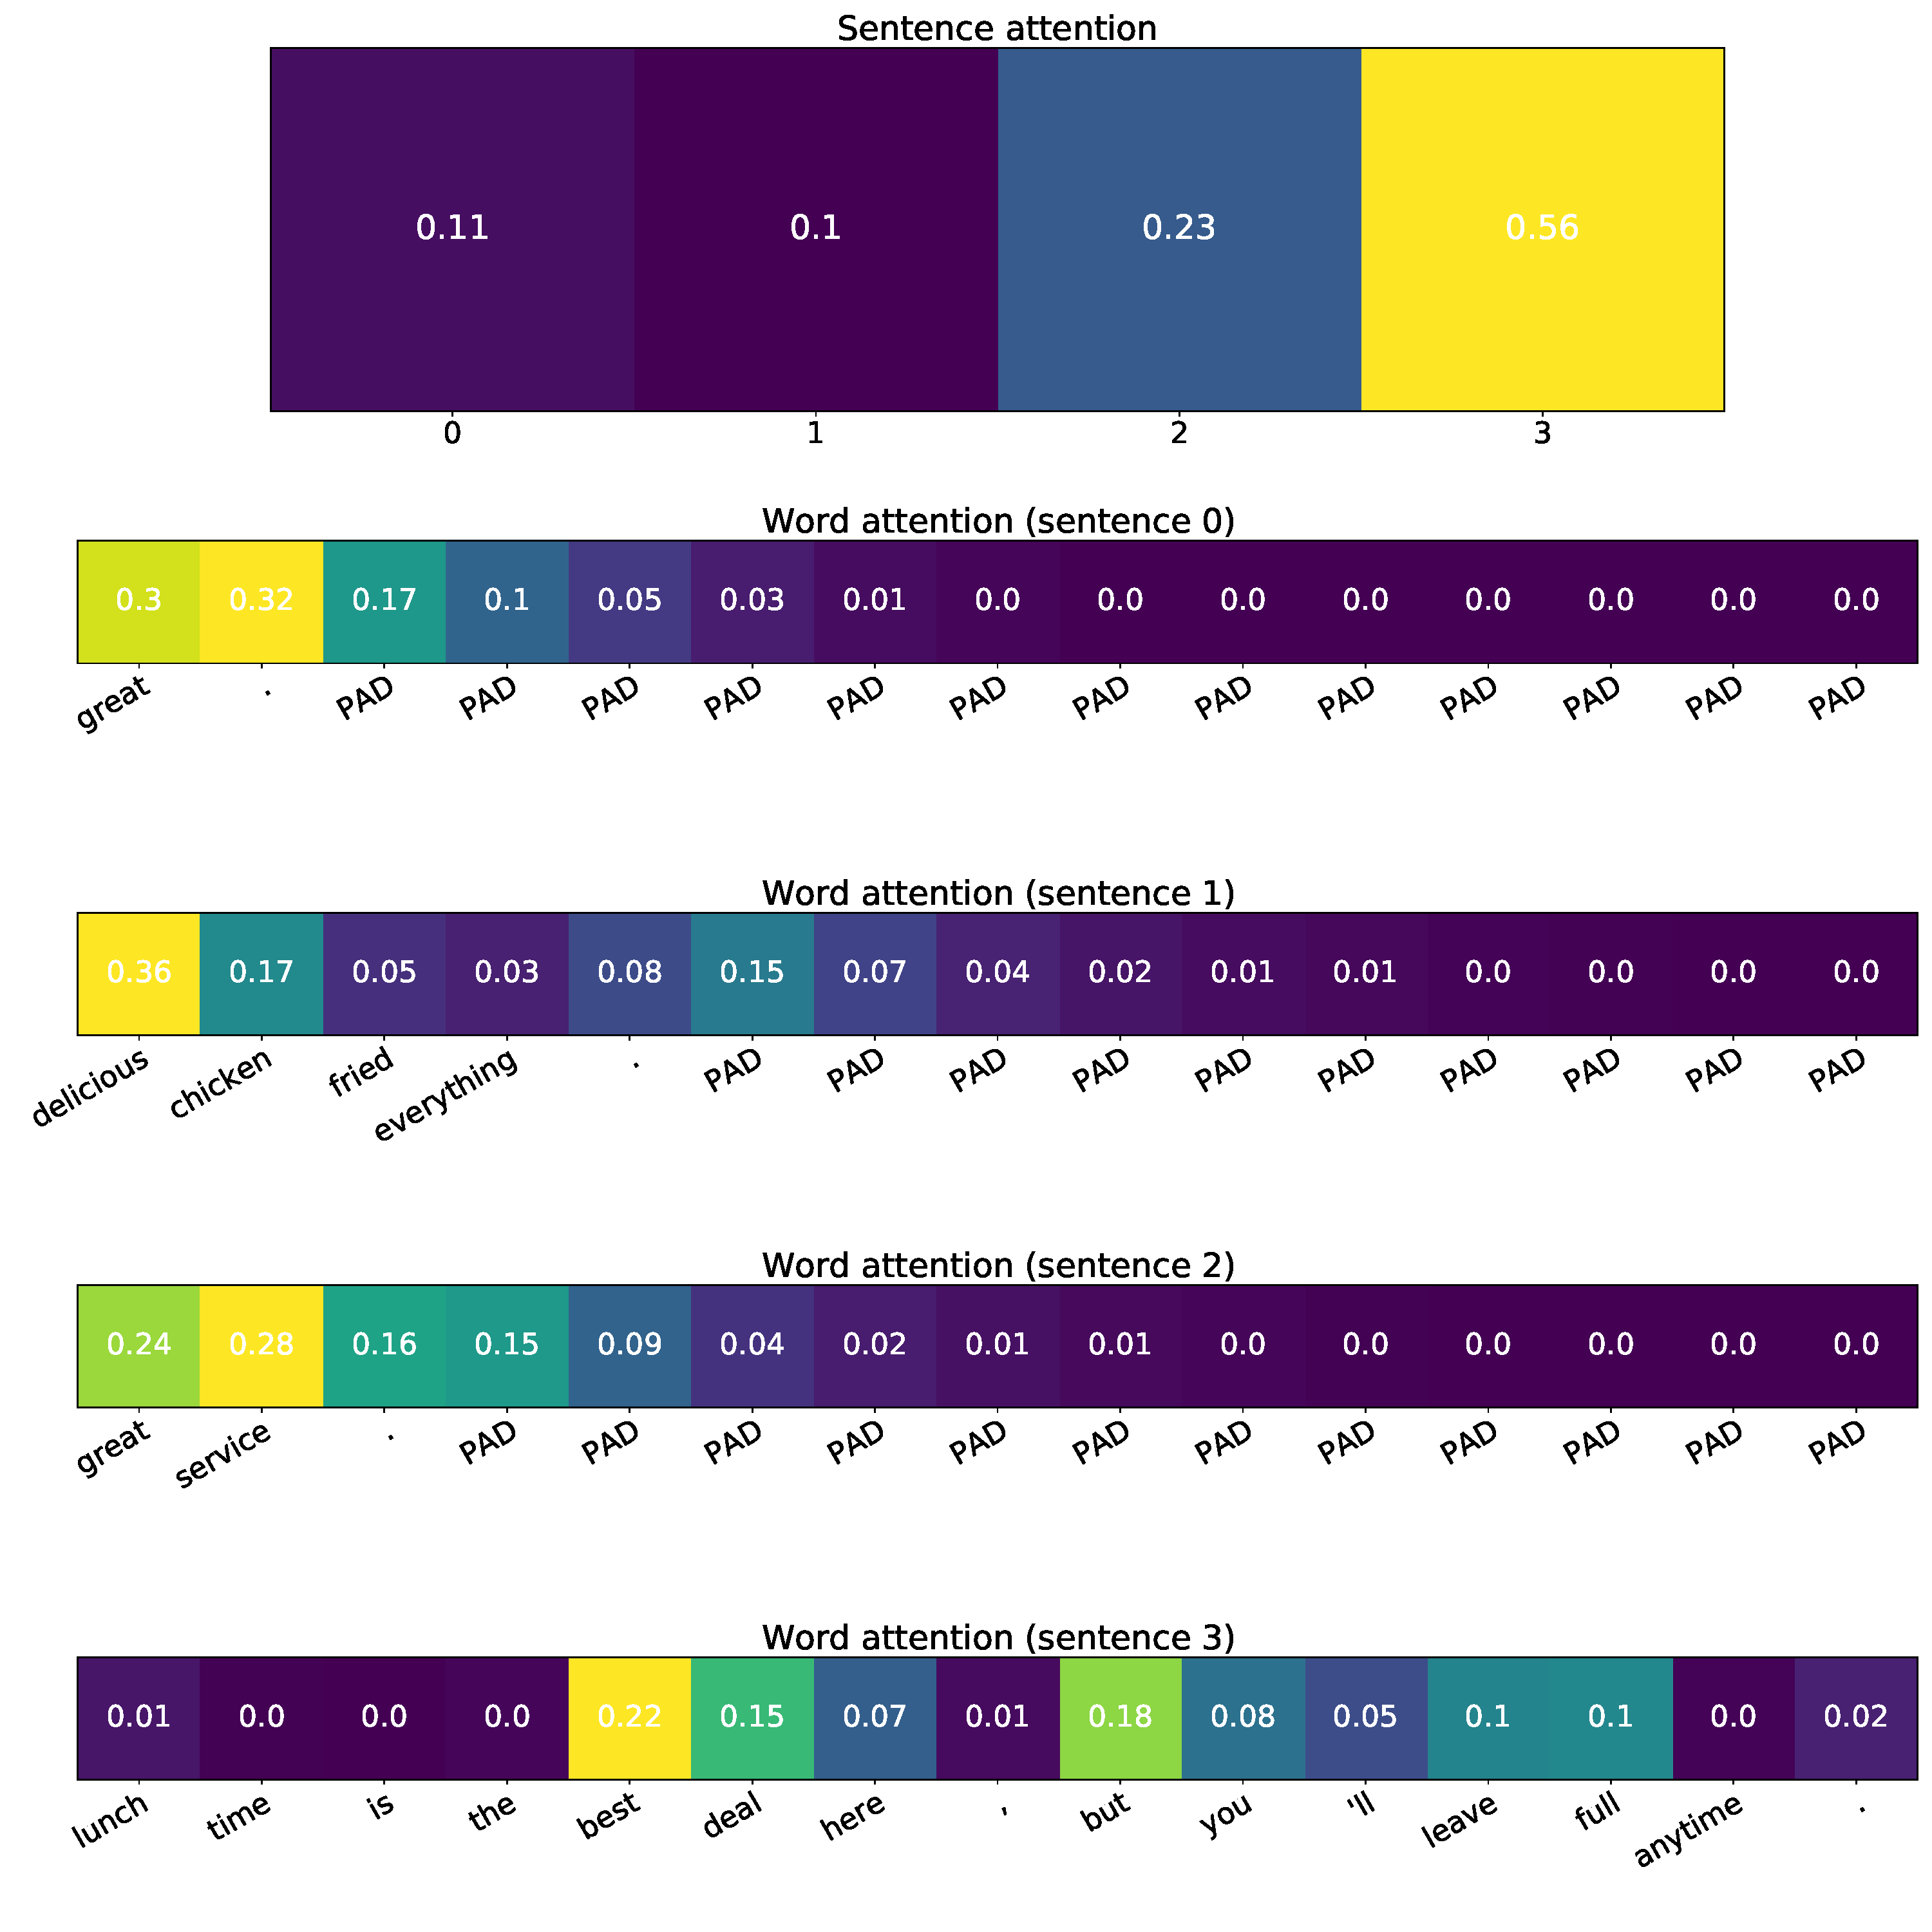
\includegraphics[scale=0.15]{img/yelp-han-visual}
\end{figure}

\end{frame}


\begin{frame}{Yahoo - Attention visualization}

\begin{figure}
\centering
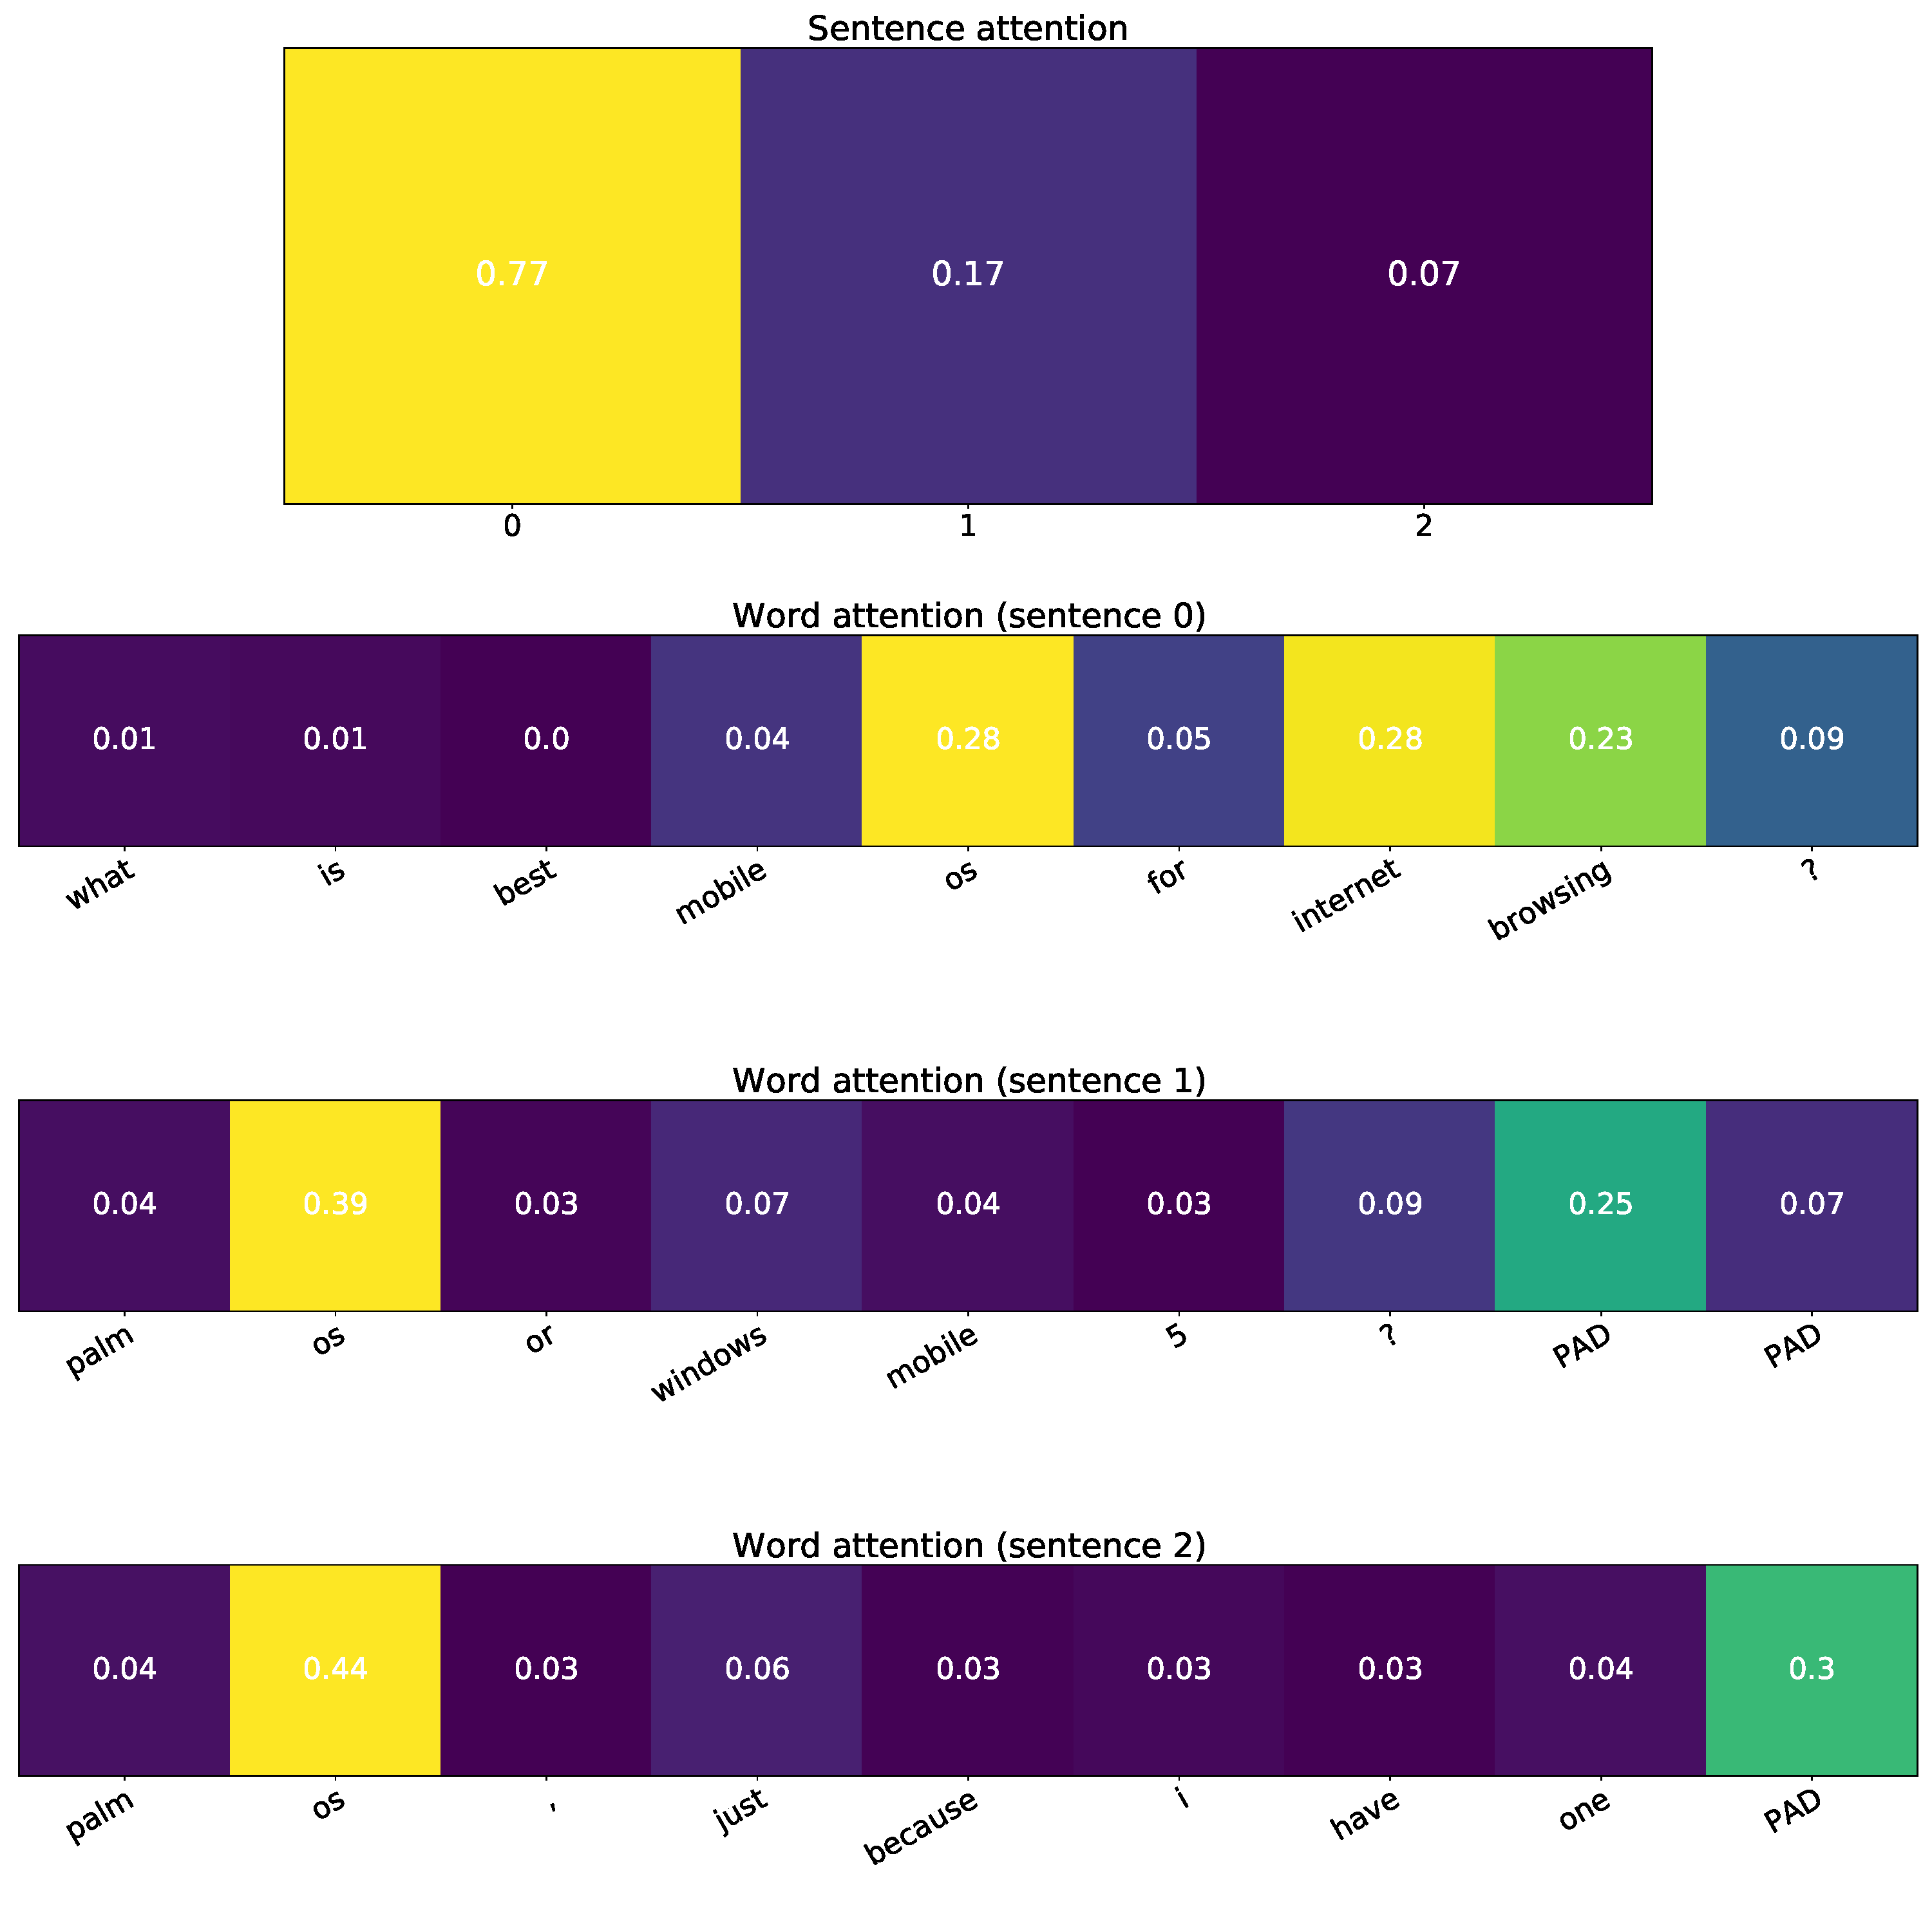
\includegraphics[scale=0.15]{img/yahoo-han-visual}
\end{figure}

\end{frame}


\begin{frame}{Amazon - Attention visualization}

\begin{figure}
\centering
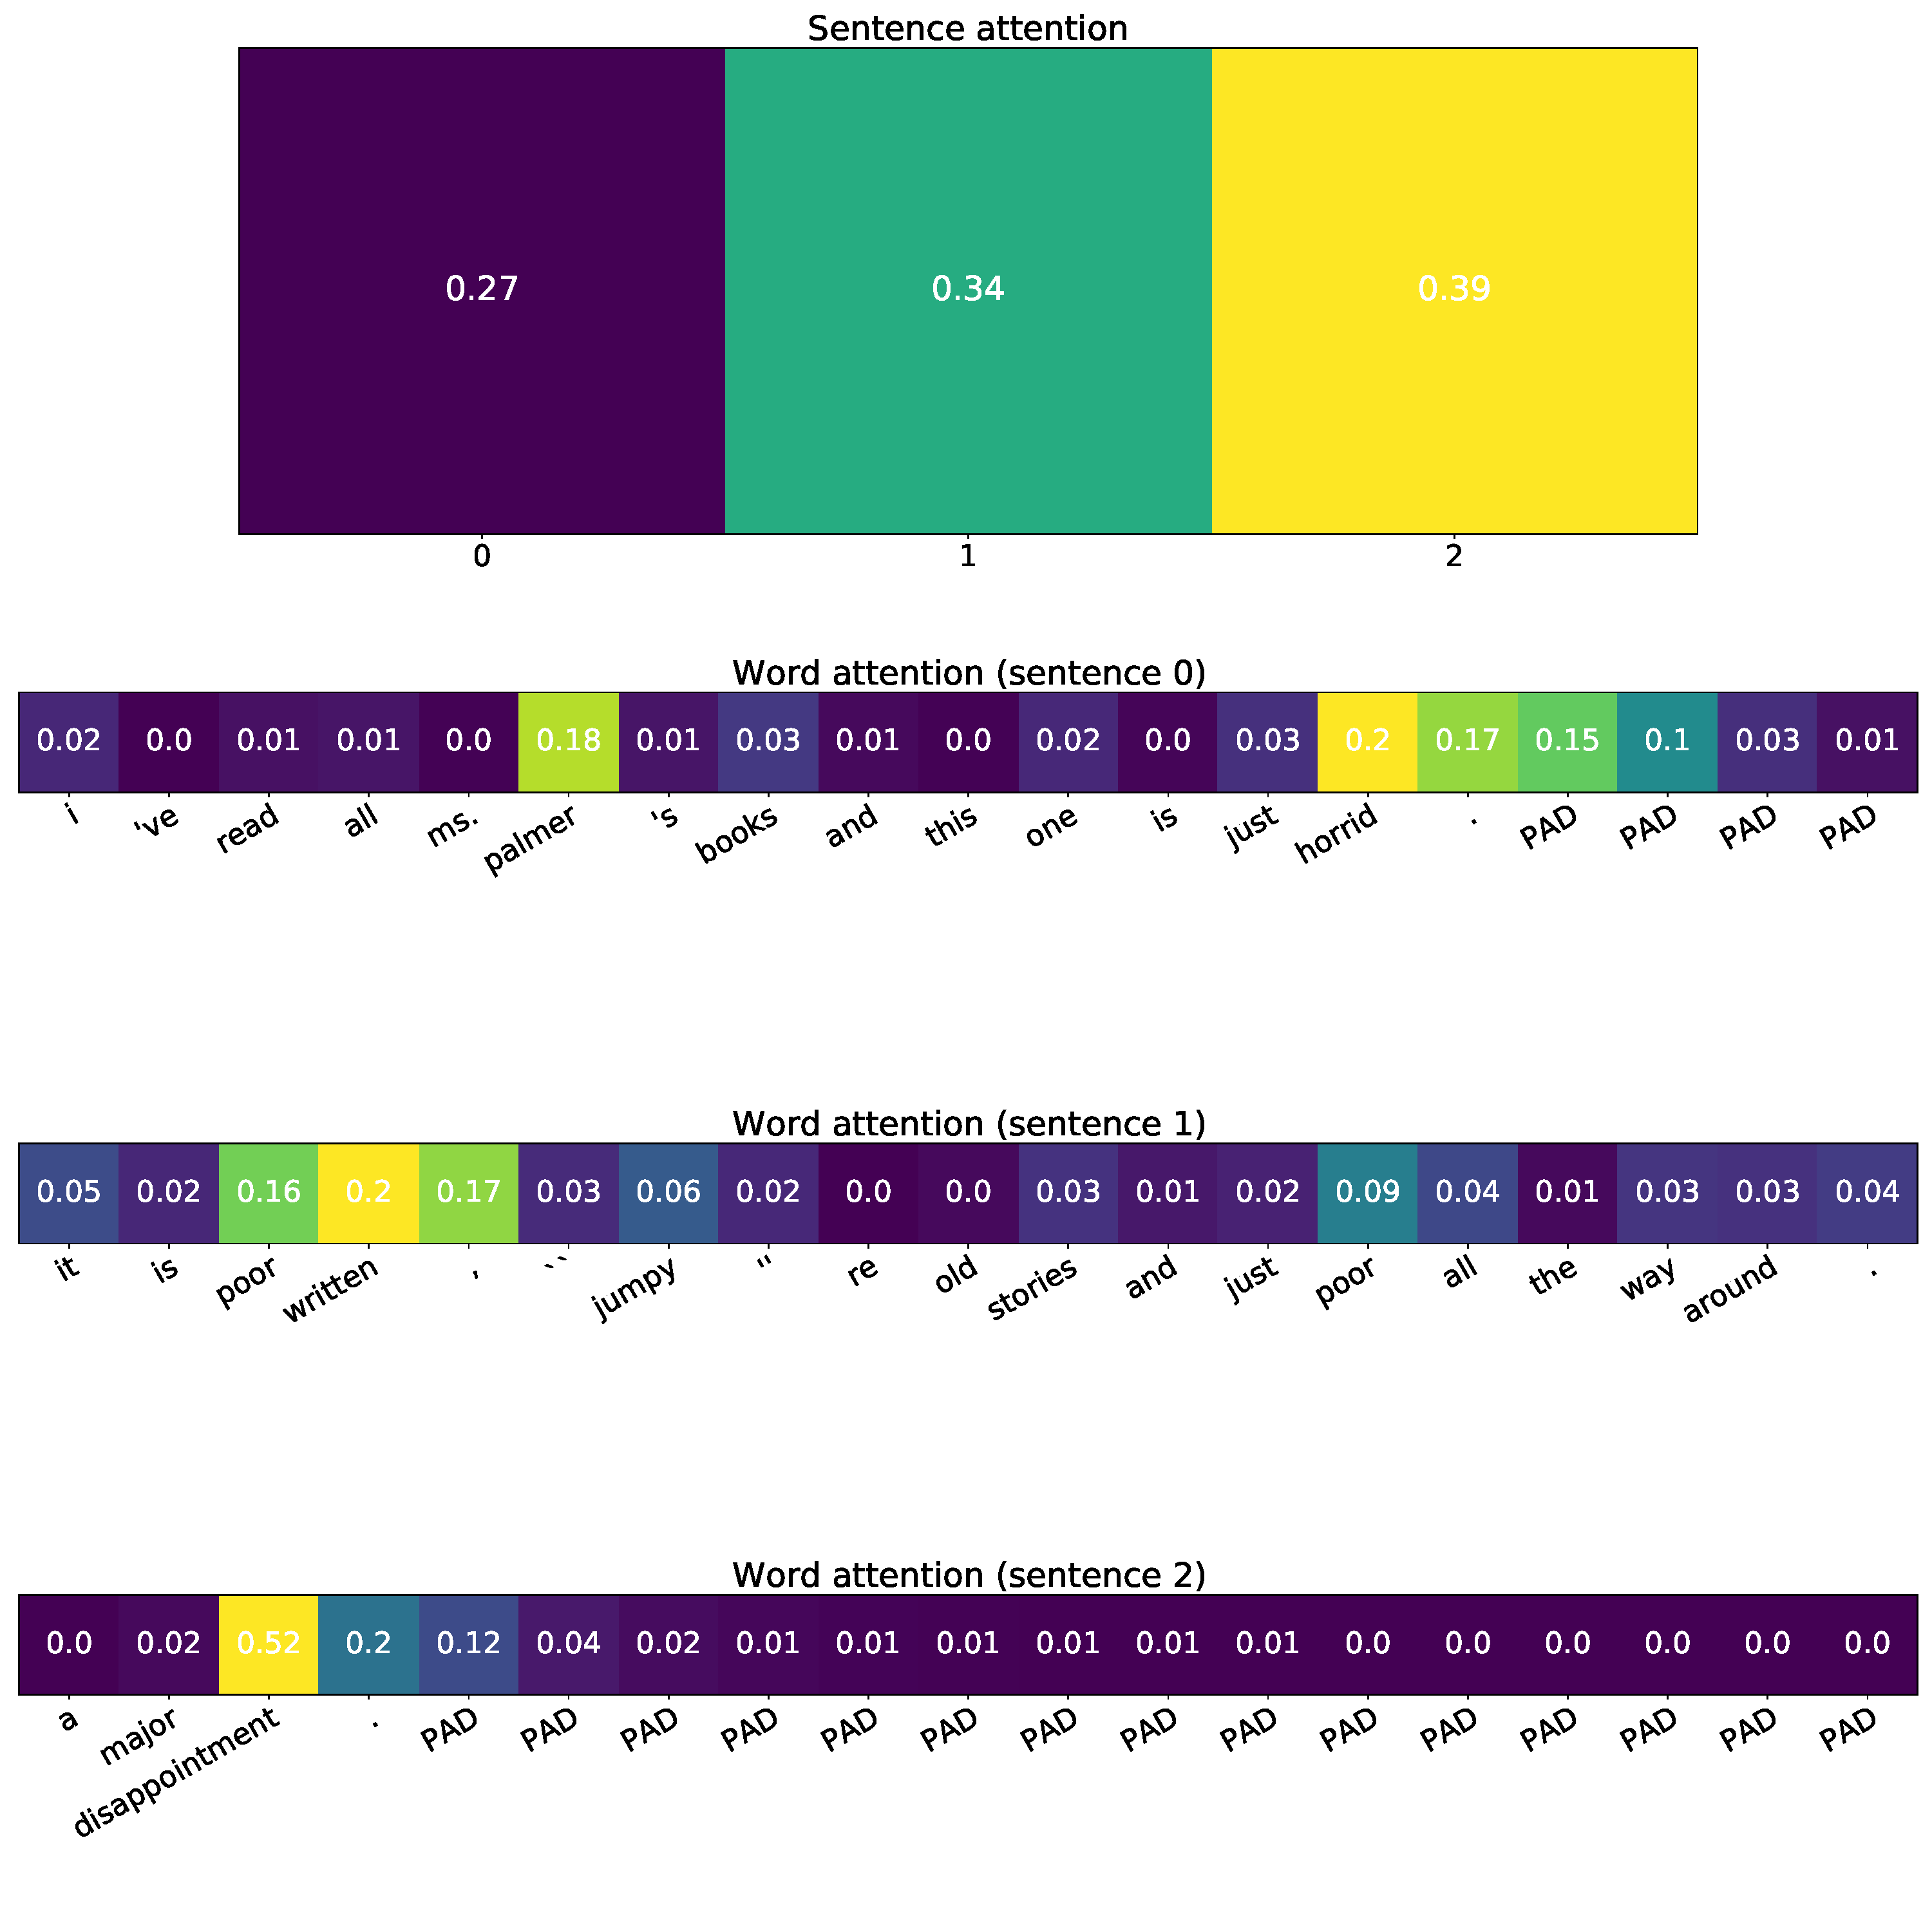
\includegraphics[scale=0.15]{img/amazon-han-visual}
\end{figure}

\end{frame}


\begin{frame}{Synthetic data set}

\begin{itemize}
\item
To verify that my model works properly, I've created a synthetic data set composed of random text. For each document, I added a keyword which is associated to a specific label.
\item
After the training, the model is always able to identify the keyword and it always predict the correct label (100\% on test set)
\end{itemize}

\end{frame}

\begin{frame}{Synthetic data set - Attention visualization}

\begin{figure}
\centering
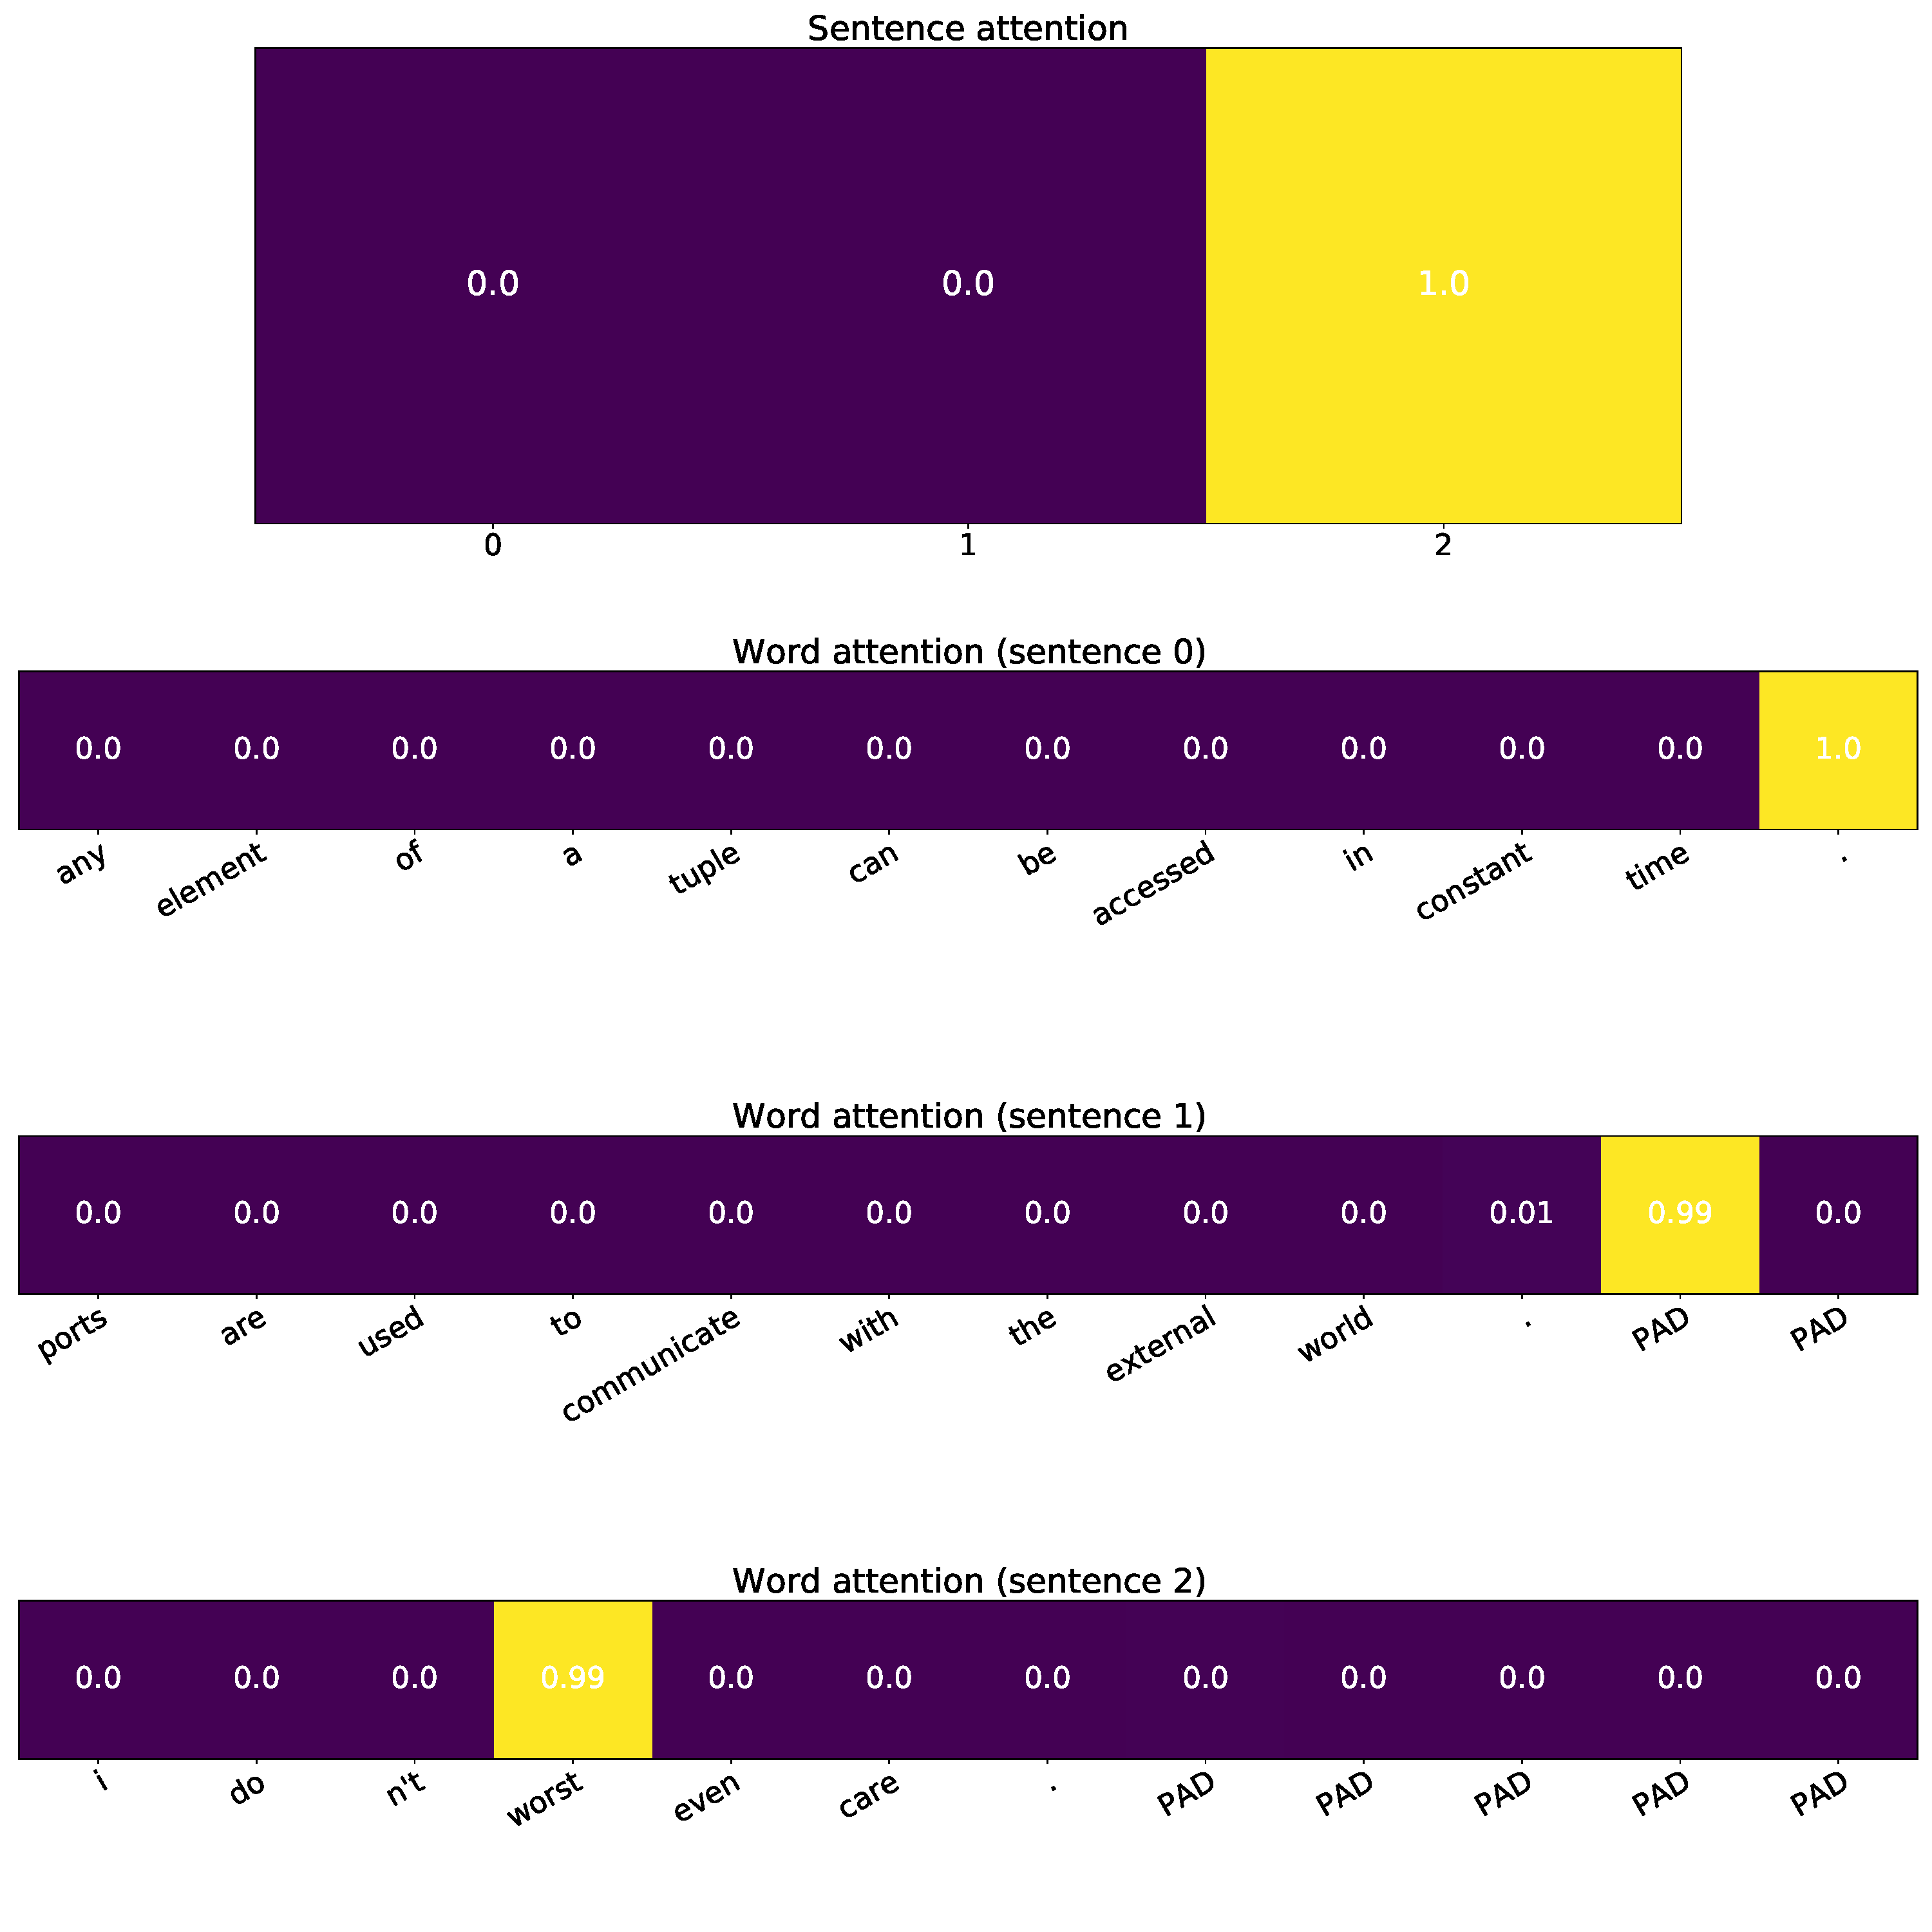
\includegraphics[scale=0.15]{img/synthetic-han-visual}
\end{figure}

\end{frame}

\begin{frame}{Conclusions}

\begin{itemize}
\item
I was able to verify that the HAN model performs better than BoW and than the flat attention.
\item
However, I wasn't able to obtain the scores reported in the paper with none of the three data sets.
\item
Maybe, it was due to the padding/cropping procedure that I had to implement to limit the computational cost.
\end{itemize}

\end{frame}


\setbeamertemplate{frame footer}{}

\begin{frame}

\begin{center}
\LARGE
Thanks for your attention
\end{center}

\end{frame}


\begin{frame}[allowframebreaks]{References}

\bibliographystyle{abbrv}
\bibliography{references}

\end{frame}


\end{document}
